\documentclass[11pt]{beamer}
\usetheme{Boadilla}
\usepackage[utf8]{inputenc}
\usepackage{amsmath}
\usepackage{amsfonts}
\usepackage{amssymb}
\usepackage{hyperref}
\usepackage{tikz}

\usetikzlibrary{arrows,decorations.markings}

%\author{}
%\title{}
%\setbeamercovered{transparent} 
%\setbeamertemplate{navigation symbols}{} 
%\logo{} 
%\institute{} 
%\date{} 
%\subject{} 
\begin{document}

%\begin{frame}
%\titlepage
%\end{frame}

%\begin{frame}
%\tableofcontents
%\end{frame}



%\begin{frame}{Polynomials}
%
%\begin{minipage}{0.3\textwidth}
%
%\begin{tikzpicture}[scale=3]
%
%\coordinate (0) at (0,0);
%\coordinate (1) at (1,0);
%\coordinate (2) at (0,1);
%
%\foreach \i in {0,1}
%    \fill (\i) circle (1pt) node [below] {\i};
%
%\foreach \i in {2}
%    \fill (\i) circle (1pt) node [above] {\i};
%
%\draw (0) --(1) -- (2) -- (0);
%
%\end{tikzpicture}
%
%\end{minipage}
%\begin{minipage}{0.69\textwidth}
%
%\begin{align*}
%N_1 &= 1-x-y \\
%N_2 &= x \\
%N_3 &= y
%\end{align*}
%
%\end{minipage}
%
%\end{frame}
\begin{frame}{2D: Triangle and quadrilateral}

%\begin{minipage}{0.69\textwidth}

\centering

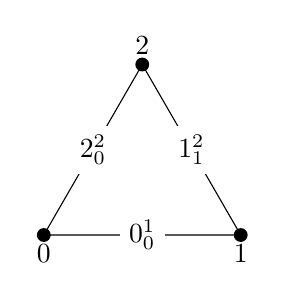
\begin{tikzpicture}[scale=2.5]

\coordinate (0) at (0,0);
\coordinate (1) at (1,0);
\coordinate (2) at (0.5,0.86603);

\foreach \i in {0,1}
    \fill (\i) circle (1pt) node [below] {\i};

\foreach \i in {2}
    \fill (\i) circle (1pt) node [above] {\i};

\draw (0) --(1) -- (2) -- (0);


\draw (0.5,  0.0)  node [fill=white, text=black] {$0_0^1$};
\draw (0.75000,   0.43301)  node [fill=white, text=black] {$1_1^2$};
\draw (0.25000,   0.43301)  node [fill=white, text=black] {$2_0^2$};

\end{tikzpicture}
\qquad
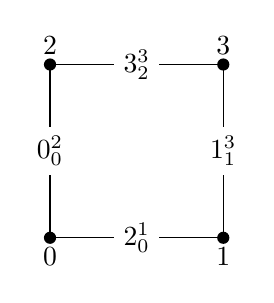
\begin{tikzpicture}[scale=2.2]

\coordinate (0) at (0,0);
\coordinate (1) at (1,0);
\coordinate (2) at (0,1);
\coordinate (3) at (1,1);

\foreach \i in {0,1}
    \fill  [text=black]  (\i) circle (1pt) node [below] {\i};

\foreach \i in {2,3}
    \fill  [text=black]  (\i) circle (1pt) node [above] {\i};

\draw (0) --(1) -- (3) -- (2) -- (0);



\draw (0.0,  0.5)  node [fill=white, text=black] {$0_0^2$};
\draw (1.0,  0.5)  node [fill=white, text=black] {$1_1^3$};
\draw (0.5,  0.0)  node [fill=white, text=black] {$2_0^1$};
\draw (0.5,  1.0)  node [fill=white, text=black] {$3_2^3$};

\end{tikzpicture}

%\end{minipage}

\end{frame}


\begin{frame}{2D: Triangle and quadrilateral - orientation}

%\begin{minipage}{0.69\textwidth}

\centering

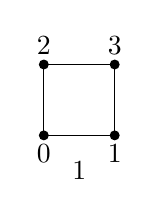
\begin{tikzpicture}[scale=0.9]

\coordinate (0) at (0,0);
\coordinate (1) at (1,0);
\coordinate (2) at (0,1);
\coordinate (3) at (1,1);

\foreach \i in {0,1}
    \fill  [text=black]  (\i) circle (2pt) node [below] {\i};

\foreach \i in {2,3}
    \fill  [text=black]  (\i) circle (2pt) node [above] {\i};

\draw (0) --(1) -- (3) -- (2) -- (0);


%\coordinate (4) at (0.2,0.2);
%\coordinate (5) at (0.8,0.2);
%\coordinate (6) at (0.2,0.8);
%\coordinate (7) at (0.8,0.8);
%
%\draw[decoration={markings,mark=at position 1 with {\arrow[scale=2,>=stealth]{>}}},postaction={decorate}] (4) --(5) -- (6) -- (7);

\node at (0.5,-0.5) {1};

\end{tikzpicture}
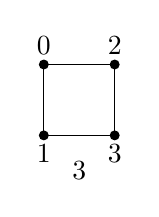
\begin{tikzpicture}[scale=0.9]

\coordinate (1) at (0,0);
\coordinate (3) at (1,0);
\coordinate (0) at (0,1);
\coordinate (2) at (1,1);

\foreach \i in {1,3}
    \fill  [text=black]  (\i) circle (2pt) node [below] {\i};

\foreach \i in {0,2}
    \fill  [text=black]  (\i) circle (2pt) node [above] {\i};

\draw (1) --(3) -- (2) -- (0) -- (1);


%\coordinate (4) at (0.2,0.2);
%\coordinate (5) at (0.8,0.2);
%\coordinate (6) at (0.2,0.8);
%\coordinate (7) at (0.8,0.8);
%
%\draw[decoration={markings,mark=at position 1 with {\arrow[scale=2,>=stealth]{>}}},postaction={decorate}] (5) --(4) -- (7) -- (6);

\node at (0.5,-0.5) {3};

\end{tikzpicture}
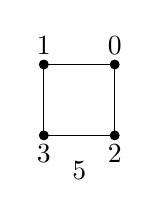
\begin{tikzpicture}[scale=0.9]

\coordinate (3) at (0,0);
\coordinate (2) at (1,0);
\coordinate (1) at (0,1);
\coordinate (0) at (1,1);

\foreach \i in {3,2}
    \fill  [text=black]  (\i) circle (2pt) node [below] {\i};

\foreach \i in {0,1}
    \fill  [text=black]  (\i) circle (2pt) node [above] {\i};

\draw (3) --(2) -- (0) -- (1) -- (3);


%\coordinate (4) at (0.2,0.2);
%\coordinate (5) at (0.8,0.2);
%\coordinate (6) at (0.2,0.8);
%\coordinate (7) at (0.8,0.8);
%
%\draw[decoration={markings,mark=at position 1 with {\arrow[scale=2,>=stealth]{>}}},postaction={decorate}] (7) --(6) -- (5) -- (4);

\node at (0.5,-0.5) {5};

\end{tikzpicture}
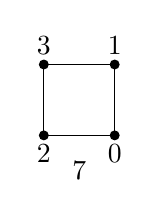
\begin{tikzpicture}[scale=0.9]

\coordinate (2) at (0,0);
\coordinate (0) at (1,0);
\coordinate (3) at (0,1);
\coordinate (1) at (1,1);

\foreach \i in {2,0}
    \fill  [text=black]  (\i) circle (2pt) node [below] {\i};

\foreach \i in {3,1}
    \fill  [text=black]  (\i) circle (2pt) node [above] {\i};

\draw (2) --(0) -- (1) -- (3) -- (2);


%\coordinate (4) at (0.2,0.2);
%\coordinate (5) at (0.8,0.2);
%\coordinate (6) at (0.2,0.8);
%\coordinate (7) at (0.8,0.8);
%
%\draw[decoration={markings,mark=at position 1 with {\arrow[scale=2,>=stealth]{>}}},postaction={decorate}] (6) --(7) -- (6) -- (7);

\node at (0.5,-0.5) {7};

\end{tikzpicture}
\quad
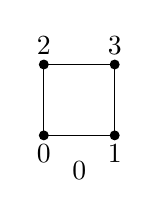
\begin{tikzpicture}[scale=0.9]

\coordinate (0) at (0,0);
\coordinate (1) at (1,0);
\coordinate (2) at (0,1);
\coordinate (3) at (1,1);

\foreach \i in {0,1}
    \fill  [text=black]  (\i) circle (2pt) node [below] {\i};

\foreach \i in {2,3}
    \fill  [text=black]  (\i) circle (2pt) node [above] {\i};

\draw (0) --(1) -- (3) -- (2) -- (0);


%\coordinate (4) at (0.2,0.2);
%\coordinate (5) at (0.8,0.2);
%\coordinate (6) at (0.2,0.8);
%\coordinate (7) at (0.8,0.8);
%
%\draw[decoration={markings,mark=at position 1 with {\arrow[scale=2,>=stealth]{>}}},postaction={decorate}] (4) --(5) -- (6) -- (7);

\node at (0.5,-0.5) {0};

\end{tikzpicture}
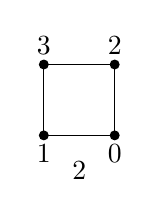
\begin{tikzpicture}[scale=0.9]

\coordinate (1) at (0,0);
\coordinate (0) at (1,0);
\coordinate (3) at (0,1);
\coordinate (2) at (1,1);

\foreach \i in {1,0}
    \fill  [text=black]  (\i) circle (2pt) node [below] {\i};

\foreach \i in {3,2}
    \fill  [text=black]  (\i) circle (2pt) node [above] {\i};

\draw (1) --(0) -- (2) -- (3) -- (1);


%\coordinate (4) at (0.2,0.2);
%\coordinate (5) at (0.8,0.2);
%\coordinate (6) at (0.2,0.8);
%\coordinate (7) at (0.8,0.8);
%
%\draw[decoration={markings,mark=at position 1 with {\arrow[scale=2,>=stealth]{>}}},postaction={decorate}] (5) --(4) -- (7) -- (6);

\node at (0.5,-0.5) {2};

\end{tikzpicture}
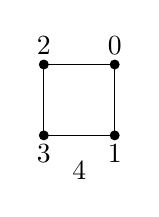
\begin{tikzpicture}[scale=0.9]

\coordinate (3) at (0,0);
\coordinate (1) at (1,0);
\coordinate (2) at (0,1);
\coordinate (0) at (1,1);

\foreach \i in {1,3}
    \fill  [text=black]  (\i) circle (2pt) node [below] {\i};

\foreach \i in {0,2}
    \fill  [text=black]  (\i) circle (2pt) node [above] {\i};

\draw (3) --(1) -- (0) -- (2) -- (3);


%\coordinate (4) at (0.2,0.2);
%\coordinate (5) at (0.8,0.2);
%\coordinate (6) at (0.2,0.8);
%\coordinate (7) at (0.8,0.8);
%
%\draw[decoration={markings,mark=at position 1 with {\arrow[scale=2,>=stealth]{>}}},postaction={decorate}] (7) --(6) -- (5) -- (4);

\node at (0.5,-0.5) {4};

\end{tikzpicture}
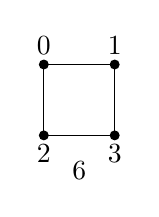
\begin{tikzpicture}[scale=0.9]

\coordinate (2) at (0,0);
\coordinate (3) at (1,0);
\coordinate (0) at (0,1);
\coordinate (1) at (1,1);

\foreach \i in {2,3}
    \fill  [text=black]  (\i) circle (2pt) node [below] {\i};

\foreach \i in {0,1}
    \fill  [text=black]  (\i) circle (2pt) node [above] {\i};

\draw (2) --(3) -- (1) -- (0) -- (2);


%\coordinate (4) at (0.2,0.2);
%\coordinate (5) at (0.8,0.2);
%\coordinate (6) at (0.2,0.8);
%\coordinate (7) at (0.8,0.8);
%
%\draw[decoration={markings,mark=at position 1 with {\arrow[scale=2,>=stealth]{>}}},postaction={decorate}] (6) --(7) -- (6) -- (7);

\node at (0.5,-0.5) {6};

\end{tikzpicture}

\vspace{0.7cm}

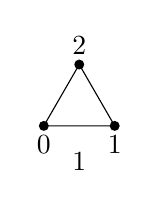
\begin{tikzpicture}[scale=0.9]

\coordinate (0) at (0,0);
\coordinate (1) at (1,0);
\coordinate (2) at (0.5,0.86603);

\foreach \i in {0,1}
    \fill (\i) circle (2pt) node [below] {\i};

\foreach \i in {2}
    \fill (\i) circle (2pt) node [above] {\i};

\draw (0) --(1) -- (2) -- (0);

\node at (0.5,-0.5) {1};

\end{tikzpicture}
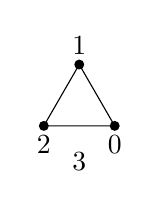
\begin{tikzpicture}[scale=0.9]

\coordinate (2) at (0,0);
\coordinate (0) at (1,0);
\coordinate (1) at (0.5,0.86603);

\foreach \i in {2,0}
    \fill (\i) circle (2pt) node [below] {\i};

\foreach \i in {1}
    \fill (\i) circle (2pt) node [above] {\i};

\draw (0) --(1) -- (2) -- (0);

\node at (0.5,-0.5) {3};

\end{tikzpicture}
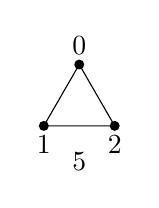
\begin{tikzpicture}[scale=0.9]

\coordinate (1) at (0,0);
\coordinate (2) at (1,0);
\coordinate (0) at (0.5,0.86603);

\foreach \i in {1, 2}
    \fill (\i) circle (2pt) node [below] {\i};

\foreach \i in {0}
    \fill (\i) circle (2pt) node [above] {\i};

\draw (0) --(1) -- (2) -- (0);

\node at (0.5,-0.5) {5};

\end{tikzpicture}
\qquad\qquad
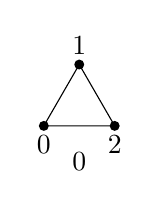
\begin{tikzpicture}[scale=0.9]

\coordinate (0) at (0,0);
\coordinate (2) at (1,0);
\coordinate (1) at (0.5,0.86603);

\foreach \i in {0,2}
    \fill (\i) circle (2pt) node [below] {\i};

\foreach \i in {1}
    \fill (\i) circle (2pt) node [above] {\i};

\draw (0) --(1) -- (2) -- (0);

\node at (0.5,-0.5) {0};

\end{tikzpicture}
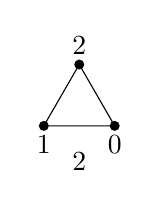
\begin{tikzpicture}[scale=0.9]

\coordinate (1) at (0,0);
\coordinate (0) at (1,0);
\coordinate (2) at (0.5,0.86603);

\foreach \i in {0,1}
    \fill (\i) circle (2pt) node [below] {\i};

\foreach \i in {2}
    \fill (\i) circle (2pt) node [above] {\i};

\draw (0) --(1) -- (2) -- (0);

\node at (0.5,-0.5) {2};

\end{tikzpicture}
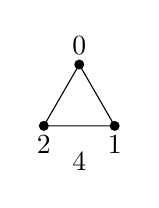
\begin{tikzpicture}[scale=0.9]

\coordinate (2) at (0,0);
\coordinate (1) at (1,0);
\coordinate (0) at (0.5,0.86603);

\foreach \i in {2,1}
    \fill (\i) circle (2pt) node [below] {\i};

\foreach \i in {0}
    \fill (\i) circle (2pt) node [above] {\i};

\draw (0) --(1) -- (2) -- (0);

\node at (0.5,-0.5) {4};

\end{tikzpicture}

%\end{minipage}

\end{frame}


%\begin{frame}{3D: Tetrahedron (currently)}
%
%\begin{minipage}{0.3\textwidth}
%
%\begin{tikzpicture}[scale=3]
%
%\coordinate (2) at (0.94281,0,-0.33333);
%\coordinate (3) at (0.47140,0.81650,-0.33333);
%\coordinate (1) at (0.47140,-0.81650,-0.33333);
%\coordinate (0) at (0,0,1);
%
%\foreach \i in {0,1,2}
%    \fill (\i) circle (1pt) node [below] {\i};
%
%\foreach \i in {3}
%    \fill (\i) circle (1pt) node [above] {\i};
%
%\draw (0) -- (1) -- (2) -- (0);
%\draw (0) -- (1) -- (3) -- (0);
%\draw (0) -- (3) -- (2) -- (0);
%
%\draw (0.23570,  -0.40825,   0.33333)  node [fill=white, text=gray] {$0_0^1$};
%\draw (0.47141,   0.00000,   0.33333)  node [fill=white, text=gray] {$1_0^2$};
%\draw (0.23570,   0.40825,   0.33333)  node [fill=white, text=gray] {$2_0^3$};
%\draw (0.70710,  -0.40825,  -0.33333)  node [fill=white, text=gray] {$3_1^2$};
%\draw (0.47140,   0.00000,  -0.33333)  node [fill=white, text=gray] {$4_1^3$};
%\draw (0.70710,   0.40825,  -0.33333)  node [fill=white, text=gray] {$5_2^3$};
%
%\end{tikzpicture}
%
%with ${\color{gray}\bullet_\bullet^\bullet}:={\color{gray}\text{line}_{\text{from}}^{\text{to}}}$
%
%\end{minipage}
%\begin{minipage}{0.69\textwidth}
%
%\centering
%
%\begin{tikzpicture}[scale=2.5]
%
%\coordinate (0) at (0,0);
%\coordinate (1) at (1,0);
%\coordinate (2) at (0.5,0.86603);
%
%\foreach \i in {0,1}
%    \fill (\i) circle (1pt) node [below] {\i};
%
%\foreach \i in {2}
%    \fill (\i) circle (1pt) node [above] {\i};
%
%\draw (0) --(1) -- (2) -- (0);
%
%
%\draw (0.5,  0.0)  node [fill=white, text=gray] {$0_0^1$};
%\draw (0.75000,   0.43301)  node [fill=white, text=gray] {$3_1^2$};
%\draw (0.25000,   0.43301)  node [fill=white, text=gray] {$1_2^0$};
%
%\end{tikzpicture}
%\begin{tikzpicture}[scale=2.5]
%
%\coordinate (1) at (0,0);
%\coordinate (0) at (1,0);
%\coordinate (3) at (0.5,0.86603);
%
%\foreach \i in {0,1}
%    \fill (\i) circle (1pt) node [below] {\i};
%
%\foreach \i in {3}
%    \fill (\i) circle (1pt) node [above] {\i};
%
%\draw (1) --(0) -- (3) -- (1);
%
%
%\draw (0.5,  0.0)  node [fill=white, text=gray] {$0_1^0$};
%\draw (0.75000,   0.43301)  node [fill=white, text=gray] {$2_0^3$};
%\draw (0.25000,   0.43301)  node [fill=white, text=gray] {$4_3^1$};
%
%\end{tikzpicture}
%
%\begin{tikzpicture}[scale=2.5]
%
%\coordinate (0) at (0,0);
%\coordinate (2) at (1,0);
%\coordinate (3) at (0.5,0.86603);
%
%\foreach \i in {0,2}
%    \fill (\i) circle (1pt) node [below] {\i};
%
%\foreach \i in {3}
%    \fill (\i) circle (1pt) node [above] {\i};
%
%\draw (0) --(2) -- (3) -- (0);
%
%
%\draw (0.5,  0.0)  node [fill=white, text=gray] {$1_0^2$};
%\draw (0.75000,   0.43301)  node [fill=white, text=gray] {$5_2^3$};
%\draw (0.25000,   0.43301)  node [fill=white, text=gray] {$2_3^0$};
%
%\end{tikzpicture}
%\begin{tikzpicture}[scale=2.5]
%
%\coordinate (2) at (0,0);
%\coordinate (1) at (1,0);
%\coordinate (3) at (0.5,0.86603);
%
%\foreach \i in {2,1}
%    \fill (\i) circle (1pt) node [below] {\i};
%
%\foreach \i in {3}
%    \fill (\i) circle (1pt) node [above] {\i};
%
%\draw (2) --(1) -- (3) -- (0);
%
%
%\draw (0.5,  0.0)  node [fill=white, text=gray] {$3_2^1$};
%\draw (0.75000,   0.43301)  node [fill=white, text=gray] {$4_1^3$};
%\draw (0.25000,   0.43301)  node [fill=white, text=gray] {$5_3^2$};
%
%\end{tikzpicture}
%
%\end{minipage}
%
%\end{frame}


\begin{frame}{3D: Tetrahedron}

\begin{minipage}{0.3\textwidth}

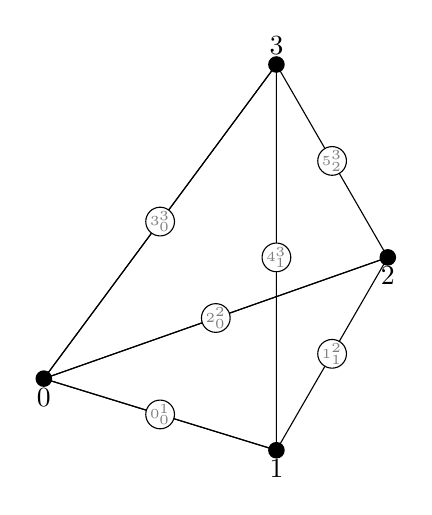
\begin{tikzpicture}[scale=3]

\coordinate (2) at (0.94281,0,-0.33333);
\coordinate (3) at (0.47140,0.81650,-0.33333);
\coordinate (1) at (0.47140,-0.81650,-0.33333);
\coordinate (0) at (0,0,1);

\foreach \i in {0,1,2}
    \fill (\i) circle (1pt) node [below] {\i};

\foreach \i in {3}
    \fill (\i) circle (1pt) node [above] {\i};

\draw (0) -- (1) -- (2) -- (0);
\draw (0) -- (1) -- (3) -- (0);
\draw (0) -- (3) -- (2) -- (0);

\draw (0.23570,  -0.40825,   0.33333)  node [inner sep=0pt,circle,fill=white!20, text=gray, draw=black] {\tiny $0_0^1$};
\draw (0.47141,   0.00000,   0.33333)  node [inner sep=0pt,circle,fill=white!20, text=gray, draw=black] {\tiny $2_0^2$};
\draw (0.23570,   0.40825,   0.33333)  node [inner sep=0pt,circle,fill=white!20, text=gray, draw=black] {\tiny $3_0^3$};
\draw (0.70710,  -0.40825,  -0.33333)  node [inner sep=0pt,circle,fill=white!20, text=gray, draw=black] {\tiny $1_1^2$};
\draw (0.47140,   0.00000,  -0.33333)  node [inner sep=0pt,circle,fill=white!20, text=gray, draw=black] {\tiny $4_1^3$};
\draw (0.70710,   0.40825,  -0.33333)  node [inner sep=0pt,circle,fill=white!20, text=gray, draw=black] {\tiny $5_2^3$};

\end{tikzpicture}

with ${\color{gray}\bullet_\bullet^\bullet}:={\color{gray}\text{line}_{\text{from}}^{\text{to}}}$

\end{minipage}
\begin{minipage}{0.69\textwidth}

\centering

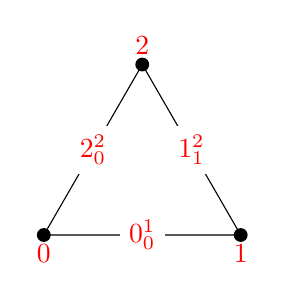
\begin{tikzpicture}[scale=2.5]

\coordinate (0) at (0,0);
\coordinate (1) at (1,0);
\coordinate (2) at (0.5,0.86603);

\foreach \i in {0,1}
    \fill [text=red] (\i) circle (1pt) node [below] {\i};

\foreach \i in {2}
    \fill [text=red] (\i) circle (1pt) node [above] {\i};

\draw (0) --(1) -- (2) -- (0);


\draw (0.5,  0.0)  node [fill=white, text=red] {$0_0^1$};
\draw (0.75000,   0.43301)  node [fill=white, text=red] {$1_1^2$};
\draw (0.25000,   0.43301)  node [fill=white, text=red] {$2_0^2$};

\end{tikzpicture}
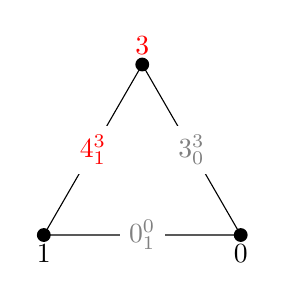
\begin{tikzpicture}[scale=2.5]

\coordinate (1) at (0,0);
\coordinate (0) at (1,0);
\coordinate (3) at (0.5,0.86603);

\foreach \i in {0,1}
    \fill (\i) circle (1pt) node [below] {\i};

\foreach \i in {3}
    \fill [text=red] (\i) circle (1pt) node [above] {\i};

\draw (1) --(0) -- (3) -- (1);


\draw (0.5,  0.0)  node [fill=white, text=gray] {$0_1^0$};
\draw (0.75000,   0.43301)  node [fill=white, text=gray] {$3_0^3$};
\draw (0.25000,   0.43301)  node [fill=white, text=red] {$4_1^3$};

\end{tikzpicture}

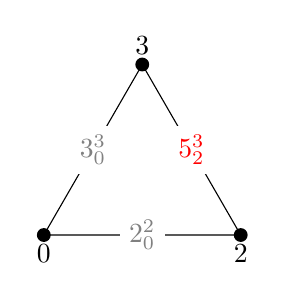
\begin{tikzpicture}[scale=2.5]

\coordinate (0) at (0,0);
\coordinate (2) at (1,0);
\coordinate (3) at (0.5,0.86603);

\foreach \i in {0,2}
    \fill (\i) circle (1pt) node [below] {\i};

\foreach \i in {3}
    \fill (\i) circle (1pt) node [above] {\i};

\draw (0) --(2) -- (3) -- (0);


\draw (0.5,  0.0)  node [fill=white, text=gray] {$2_0^2$};
\draw (0.75000,   0.43301)  node [fill=white, text=red] {$5_2^3$};
\draw (0.25000,   0.43301)  node [fill=white, text=gray] {$3_0^3$};

\end{tikzpicture}
\begin{tikzpicture}[scale=2.5]

\coordinate (2) at (0,0);
\coordinate (1) at (1,0);
\coordinate (3) at (0.5,0.86603);

\foreach \i in {2,1}
    \fill (\i) circle (1pt) node [below] {\i};

\foreach \i in {3}
    \fill (\i) circle (1pt) node [above] {\i};

\draw (2) --(1) -- (3) -- (0);


\draw (0.5,  0.0)  node [fill=white, text=gray] {$1_2^1$};
\draw (0.75000,   0.43301)  node [fill=white, text=gray] {$4_1^3$};
\draw (0.25000,   0.43301)  node [fill=white, text=gray] {$5_2^3$};

\end{tikzpicture}

\end{minipage}

\end{frame}

\begin{frame}{3D: Pyramid}

\begin{minipage}{0.3\textwidth}

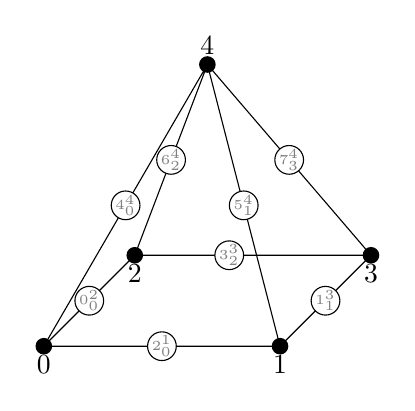
\begin{tikzpicture}[scale=3]

\coordinate (0) at (0,0,1);
\coordinate (1) at (1,0,1);
\coordinate (2) at (0,0,0);
\coordinate (3) at (1,0,0);
\coordinate (4) at (0.5,1,0.5);

\foreach \i in {0,1,2,3}
    \fill (\i) circle (1pt) node [below] {\i};

\foreach \i in {4}
    \fill (\i) circle (1pt) node [above] {\i};

\draw (0) -- (1) -- (3) -- (2) -- (0);
\draw (1) -- (4) -- (3);
\draw (0) -- (4) -- (2);

\draw (0, 0, 0.5)  node [inner sep=0pt,circle,fill=white!20, text=gray, draw=black] {\tiny $0_0^2$};
\draw (1, 0, 0.5)  node [inner sep=0pt,circle,fill=white!20, text=gray, draw=black] {\tiny $1_1^3$};

\draw (0.5, 0, 1)  node [inner sep=0pt,circle,fill=white!20, text=gray, draw=black] {\tiny $2_0^1$};
\draw (0.4, 0, 0)  node [inner sep=0pt,circle,fill=white!20, text=gray, draw=black] {\tiny $3_2^3$};


\draw (0.25000, 0.50000, 0.75000)  node [inner sep=0pt,circle,fill=white!20, text=gray, draw=black] {\tiny $4_0^4$};
\draw (0.75000, 0.50000, 0.75000)  node [inner sep=0pt,circle,fill=white!20, text=gray, draw=black] {\tiny $5_1^4$};
\draw (0.25000, 0.50000, 0.25000)  node [inner sep=0pt,circle,fill=white!20, text=gray, draw=black] {\tiny $6_2^4$};
\draw (0.75000, 0.50000, 0.25000)  node [inner sep=0pt,circle,fill=white!20, text=gray, draw=black] {\tiny $7_3^4$};

%\draw (0.47141,   0.00000,   0.33333)  node [fill=white, text=gray] {\footnotesize $2_0^2$};
%\draw (0.23570,   0.40825,   0.33333)  node [fill=white, text=gray] {\footnotesize $3_0^3$};
%\draw (0.70710,  -0.40825,  -0.33333)  node [fill=white, text=gray] {\footnotesize $1_1^2$};
%\draw (0.47140,   0.00000,  -0.33333)  node [fill=white, text=gray] {\footnotesize $4_1^3$};
%\draw (0.70710,   0.40825,  -0.33333)  node [fill=white, text=gray] {\footnotesize $5_2^3$};

\end{tikzpicture}

with ${\color{gray}\bullet_\bullet^\bullet}:={\color{gray}\text{line}_{\text{from}}^{\text{to}}}$

\end{minipage}
\begin{minipage}{0.69\textwidth}

\centering


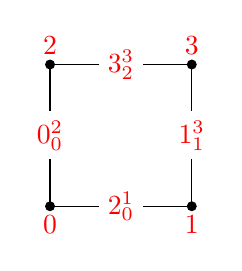
\begin{tikzpicture}[scale=1.8]

\coordinate (0) at (0,0);
\coordinate (1) at (1,0);
\coordinate (2) at (0,1);
\coordinate (3) at (1,1);

\foreach \i in {0,1}
    \fill  [text=red]  (\i) circle (1pt) node [below] {\i};

\foreach \i in {2,3}
    \fill  [text=red]  (\i) circle (1pt) node [above] {\i};

\draw (0) --(1) -- (3) -- (2) -- (0);



\draw (0.0,  0.5)  node [fill=white, text=red] {$0_0^2$};
\draw (1.0,  0.5)  node [fill=white, text=red] {$1_1^3$};
\draw (0.5,  0.0)  node [fill=white, text=red] {$2_0^1$};
\draw (0.5,  1.0)  node [fill=white, text=red] {$3_2^3$};

\end{tikzpicture}
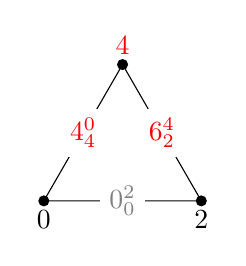
\begin{tikzpicture}[scale=2.0]

\coordinate (0) at (0,0);
\coordinate (2) at (1,0);
\coordinate (4) at (0.5,0.86603);

\foreach \i in {0,2}
    \fill (\i) circle (1pt) node [below] {\i};

\foreach \i in {4}
    \fill [text=red] (\i) circle (1pt) node [above] {\i};

\draw (0) --(2) -- (4) -- (0);


\draw (0.5,  0.0)  node [fill=white, text=gray] {$0_0^2$};
\draw (0.75000,   0.43301)  node [fill=white, text=red] {$6_2^4$};
\draw (0.25000,   0.43301)  node [fill=white, text=red] {$4_4^0$};

\end{tikzpicture}
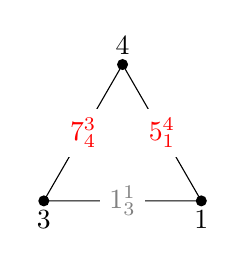
\begin{tikzpicture}[scale=2.0]

\coordinate (3) at (0,0);
\coordinate (1) at (1,0);
\coordinate (4) at (0.5,0.86603);

\foreach \i in {3,1}
    \fill (\i) circle (1pt) node [below] {\i};

\foreach \i in {4}
    \fill (\i) circle (1pt) node [above] {\i};

\draw (3) --(1) -- (4) -- (3);


\draw (0.5,  0.0)  node [fill=white, text=gray] {$1_3^1$};
\draw (0.75000,   0.43301)  node [fill=white, text=red] {$5_1^4$};
\draw (0.25000,   0.43301)  node [fill=white, text=red] {$7_4^3$};

\end{tikzpicture}

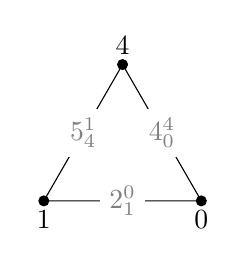
\begin{tikzpicture}[scale=2.0]

\coordinate (1) at (0,0);
\coordinate (0) at (1,0);
\coordinate (4) at (0.5,0.86603);

\foreach \i in {1,0}
    \fill (\i) circle (1pt) node [below] {\i};

\foreach \i in {4}
    \fill (\i) circle (1pt) node [above] {\i};

\draw (1) --(0) -- (4) -- (1);


\draw (0.5,  0.0)  node [fill=white, text=gray] {$2_1^0$};
\draw (0.75000,   0.43301)  node [fill=white, text=gray] {$4_0^4$};
\draw (0.25000,   0.43301)  node [fill=white, text=gray] {$5_4^1$};

\end{tikzpicture}
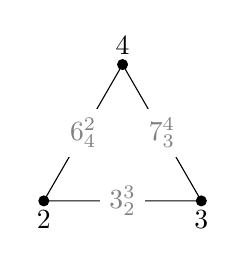
\begin{tikzpicture}[scale=2.0]

\coordinate (2) at (0,0);
\coordinate (3) at (1,0);
\coordinate (4) at (0.5,0.86603);

\foreach \i in {2,3}
    \fill (\i) circle (1pt) node [below] {\i};

\foreach \i in {4}
    \fill (\i) circle (1pt) node [above] {\i};

\draw (2) --(3) -- (4) -- (2);


\draw (0.5,  0.0)  node [fill=white, text=gray] {$3_2^3$};
\draw (0.75000,   0.43301)  node [fill=white, text=gray] {$7_3^4$};
\draw (0.25000,   0.43301)  node [fill=white, text=gray] {$6_4^2$};

\end{tikzpicture}

\end{minipage}

\end{frame}

\begin{frame}{3D: Wedge}

\begin{minipage}{0.3\textwidth}

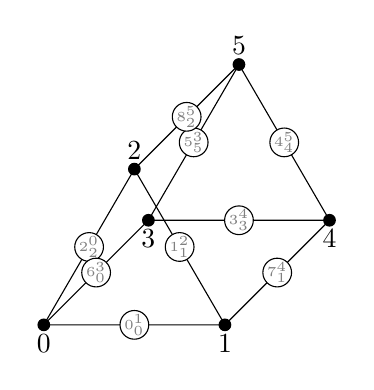
\begin{tikzpicture}[scale=2.3]

\coordinate (0) at (0,0,1.5);
\coordinate (1) at (1,0,1.5);
\coordinate (2) at (0.5,0.86,1.5);

\coordinate (3) at (0,0,0);
\coordinate (4) at (1,0,0);
\coordinate (5) at (0.5,0.86,0);

\foreach \i in {0,1,3,4}
    \fill (\i) circle (1pt) node [below] {\i};

\foreach \i in {2,5}
    \fill (\i) circle (1pt) node [above] {\i};

\draw (0) -- (1) -- (2) -- (0);
\draw (3) -- (4) -- (5) -- (3);
\draw (0) -- (3);
\draw (1) -- (4);
\draw (2) -- (5);
%\draw (1) -- (4) -- (3);
%\draw (0) -- (4) -- (2);

%\draw (0.23570,  -0.40825,   0.33333)  node [fill=white, text=gray] {$0_0^1$};
%\draw (0.47141,   0.00000,   0.33333)  node [fill=white, text=gray] {$1_0^2$};
%\draw (0.23570,   0.40825,   0.33333)  node [fill=white, text=gray] {$2_0^3$};
%\draw (0.70710,  -0.40825,  -0.33333)  node [fill=white, text=gray] {$3_1^2$};
%\draw (0.47140,   0.00000,  -0.33333)  node [fill=white, text=gray] {$4_1^3$};
%\draw (0.70710,   0.40825,  -0.33333)  node [fill=white, text=gray] {$5_2^3$};

\draw (0.50, 0.00, 1.5)  node [inner sep=0pt,circle,fill=white!20, text=gray, draw=black] {\tiny $0_0^1$};
\draw (0.75, 0.43, 1.5)  node [inner sep=0pt,circle,fill=white!20, text=gray, draw=black] {\tiny $1_1^2$};
\draw (0.25, 0.43, 1.5)  node [inner sep=0pt,circle,fill=white!20, text=gray, draw=black] {\tiny $2_2^0$};

\draw (0.50, 0.00, 0.0)  node [inner sep=0pt,circle,fill=white!20, text=gray, draw=black] {\tiny $3_3^4$};
\draw (0.75, 0.43, 0.0)  node [inner sep=0pt,circle,fill=white!20, text=gray, draw=black] {\tiny $4_4^5$};
\draw (0.25, 0.43, 0.0)  node [inner sep=0pt,circle,fill=white!20, text=gray, draw=black] {\tiny $5_5^3$};


\draw (0.00, 0.00, 0.75)  node [inner sep=0pt,circle,fill=white!20, text=gray, draw=black] {\tiny $6_0^3$};
\draw (1.00, 0.00, 0.75)  node [inner sep=0pt,circle,fill=white!20, text=gray, draw=black] {\tiny $7_1^4$};
\draw (0.50, 0.86, 0.75)  node [inner sep=0pt,circle,fill=white!20, text=gray, draw=black] {\tiny $8_2^5$};


\end{tikzpicture}

with ${\color{gray}\bullet_\bullet^\bullet}:={\color{gray}\text{line}_{\text{from}}^{\text{to}}}$

\end{minipage}
\begin{minipage}{0.69\textwidth}

\centering


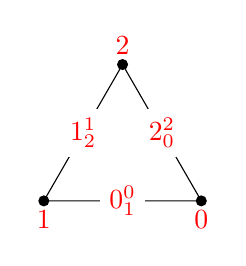
\begin{tikzpicture}[scale=2.0]

\coordinate (1) at (0,0);
\coordinate (0) at (1,0);
\coordinate (2) at (0.5,0.86603);

\foreach \i in {0,1}
    \fill [text=red] (\i) circle (1pt) node [below] {\i};

\foreach \i in {2}
    \fill [text=red] (\i) circle (1pt) node [above] {\i};

\draw (1) --(0) -- (2) -- (1);


\draw (0.50000,  0.00000)  node [fill=white, text=red] {$0_1^0$};
\draw (0.75000,  0.43301)  node [fill=white, text=red] {$2_0^2$};
\draw (0.25000,  0.43301)  node [fill=white, text=red] {$1_2^1$};

\end{tikzpicture}
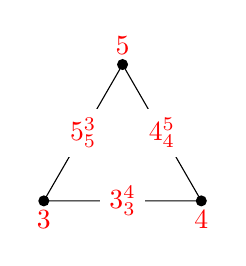
\begin{tikzpicture}[scale=2.0]

\coordinate (3) at (0,0);
\coordinate (4) at (1,0);
\coordinate (5) at (0.5,0.86603);

\foreach \i in {3,4}
    \fill [text=red] (\i) circle (1pt) node [below] {\i};

\foreach \i in {5}
    \fill [text=red] (\i) circle (1pt) node [above] {\i};

\draw (3) --(4) -- (5) -- (3);


\draw (0.50000,  0.00000)  node [fill=white, text=red] {$3_3^4$};
\draw (0.75000,  0.43301)  node [fill=white, text=red] {$4_4^5$};
\draw (0.25000,  0.43301)  node [fill=white, text=red] {$5_5^3$};

\end{tikzpicture}

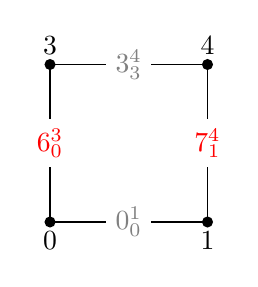
\begin{tikzpicture}[scale=2.0]

\coordinate (0) at (0,0);
\coordinate (1) at (1,0);
\coordinate (3) at (0,1);
\coordinate (4) at (1,1);

\foreach \i in {0,1}
    \fill  [text=black]  (\i) circle (1pt) node [below] {\i};

\foreach \i in {3,4}
    \fill  [text=black]  (\i) circle (1pt) node [above] {\i};

\draw (0) --(1) -- (4) -- (3) -- (0);



\draw (0.0,  0.5)  node [fill=white, text=red] {$6_0^3$};
\draw (1.0,  0.5)  node [fill=white, text=red] {$7_1^4$};
\draw (0.5,  0.0)  node [fill=white, text=gray] {$0_0^1$};
\draw (0.5,  1.0)  node [fill=white, text=gray] {$3_3^4$};

\end{tikzpicture}
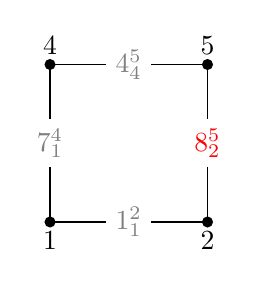
\begin{tikzpicture}[scale=2.0]

\coordinate (1) at (0,0);
\coordinate (2) at (1,0);
\coordinate (4) at (0,1);
\coordinate (5) at (1,1);

\foreach \i in {1,2}
    \fill  [text=black]  (\i) circle (1pt) node [below] {\i};

\foreach \i in {4,5}
    \fill  [text=black]  (\i) circle (1pt) node [above] {\i};

\draw (1) --(2) -- (5) -- (4) -- (1);



\draw (0.0,  0.5)  node [fill=white, text=gray] {$7_1^4$};
\draw (1.0,  0.5)  node [fill=white, text=red] {$8_2^5$};
\draw (0.5,  0.0)  node [fill=white, text=gray] {$1_1^2$};
\draw (0.5,  1.0)  node [fill=white, text=gray] {$4_4^5$};

\end{tikzpicture}
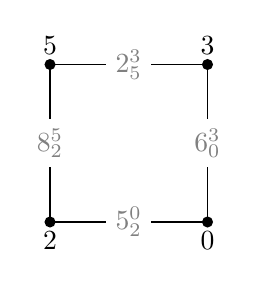
\begin{tikzpicture}[scale=2.0]

\coordinate (2) at (0,0);
\coordinate (0) at (1,0);
\coordinate (5) at (0,1);
\coordinate (3) at (1,1);

\foreach \i in {0,2}
    \fill  [text=black]  (\i) circle (1pt) node [below] {\i};

\foreach \i in {3,5}
    \fill  [text=black]  (\i) circle (1pt) node [above] {\i};

\draw (2) --(0) -- (3) -- (5) -- (2);



\draw (0.0,  0.5)  node [fill=white, text=gray] {$8_2^5$};
\draw (1.0,  0.5)  node [fill=white, text=gray] {$6_0^3$};
\draw (0.5,  0.0)  node [fill=white, text=gray] {$5_2^0$};
\draw (0.5,  1.0)  node [fill=white, text=gray] {$2_5^3$};

\end{tikzpicture}

\end{minipage}

\end{frame}

\begin{frame}{3D: Hexahedron}

\begin{minipage}{0.3\textwidth}

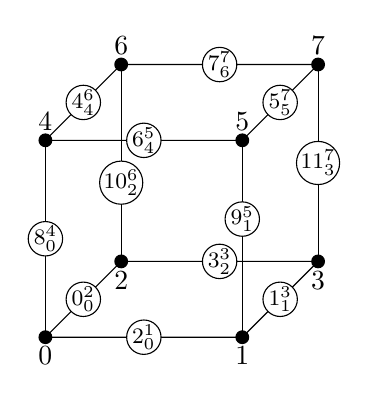
\begin{tikzpicture}[scale=2.5]

\coordinate (0) at (0,0,1);
\coordinate (1) at (1,0,1);
\coordinate (2) at (0,0,0);
\coordinate (3) at (1,0,0);

\coordinate (4) at (0,1,1);
\coordinate (5) at (1,1,1);
\coordinate (6) at (0,1,0);
\coordinate (7) at (1,1,0);

\foreach \i in {0,1,2,3}
    \fill (\i) circle (1pt) node [below] {\i};

\foreach \i in {4,5,6,7}
    \fill (\i) circle (1pt) node [above] {\i};

\draw (0) -- (1) -- (3) -- (2) -- (0);
\draw (4) -- (5) -- (7) -- (6) -- (4);
\draw (0) -- (4);
\draw (1) -- (5);
\draw (2) -- (6);
\draw (3) -- (7);
%\draw (1) -- (4) -- (3);
%\draw (0) -- (4) -- (2);

%\draw (0.23570,  -0.40825,   0.33333)  node [fill=white, text=gray] {$0_0^1$};
%\draw (0.47141,   0.00000,   0.33333)  node [fill=white, text=gray] {$1_0^2$};
%\draw (0.23570,   0.40825,   0.33333)  node [fill=white, text=gray] {$2_0^3$};
%\draw (0.70710,  -0.40825,  -0.33333)  node [fill=white, text=gray] {$3_1^2$};
%\draw (0.47140,   0.00000,  -0.33333)  node [fill=white, text=gray] {$4_1^3$};
%\draw (0.70710,   0.40825,  -0.33333)  node [fill=white, text=gray] {$5_2^3$};


\draw (0.0, 0.0, 0.5)  node [inner sep=0pt,circle,fill=white!20, draw=black] {\footnotesize $0_0^2$};
\draw (1.0, 0.0, 0.5)  node [inner sep=0pt,circle,fill=white!20, draw=black] {\footnotesize $1_1^3$};
\draw (0.5, 0.0, 1.0)  node [inner sep=0pt,circle,fill=white!20, draw=black] {\footnotesize $2_0^1$};
\draw (0.5, 0.0, 0.0)  node [inner sep=0pt,circle,fill=white!20, draw=black] {\footnotesize $3_2^3$};

\draw (0.0, 1.0, 0.5)  node [inner sep=0pt,circle,fill=white!20, draw=black] {\footnotesize $4_4^6$};
\draw (1.0, 1.0, 0.5)  node [inner sep=0pt,circle,fill=white!20, draw=black] {\footnotesize $5_5^7$};
\draw (0.5, 1.0, 1.0)  node [inner sep=0pt,circle,fill=white!20, draw=black] {\footnotesize $6_4^5$};
\draw (0.5, 1.0, 0.0)  node [inner sep=0pt,circle,fill=white!20, draw=black] {\footnotesize $7_6^7$};

\draw (0.0, 0.5, 1.0)  node [inner sep=0pt,circle,fill=white!20, draw=black] {\footnotesize $8_0^4$};
\draw (1.0, 0.6, 1.0)  node [inner sep=0pt,circle,fill=white!20, draw=black] {\footnotesize $9_1^5$};
\draw (0.0, 0.4, 0.0)  node [inner sep=0pt,circle,fill=white!20, draw=black] {\footnotesize $10_2^6$};
\draw (1.0, 0.5, 0.0)  node [inner sep=0pt,circle,fill=white!20, draw=black] {\footnotesize $11_3^7$};

\end{tikzpicture}

with ${\color{gray}\bullet_\bullet^\bullet}:={\color{gray}\text{line}_{\text{from}}^{\text{to}}}$

\end{minipage}
\begin{minipage}{0.69\textwidth}

\centering

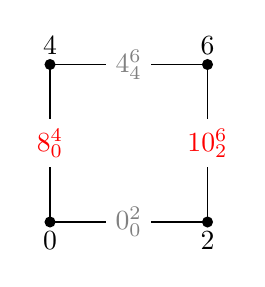
\begin{tikzpicture}[scale=2.0]

\coordinate (0) at (0,0);
\coordinate (2) at (1,0);
\coordinate (4) at (0,1);
\coordinate (6) at (1,1);

\foreach \i in {0,2}
    \fill (\i) circle (1pt) node [below] {\i};

\foreach \i in {4,6}
    \fill (\i) circle (1pt) node [above] {\i};

\draw (0) --(2) -- (6) -- (4) -- (0);



\draw (0.0,  0.5)  node [fill=white, text=red] {$8_0^4$};
\draw (1.0,  0.5)  node [fill=white, text=red] {$10_2^6$};
\draw (0.5,  0.0)  node [fill=white, text=gray] {$0_0^2$};
\draw (0.5,  1.0)  node [fill=white, text=gray] {$4_4^6$};

\end{tikzpicture}
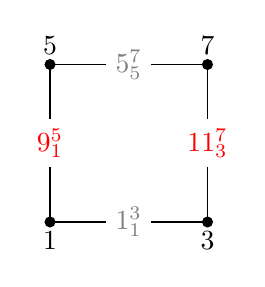
\begin{tikzpicture}[scale=2.0]

\coordinate (1) at (0,0);
\coordinate (3) at (1,0);
\coordinate (5) at (0,1);
\coordinate (7) at (1,1);

\foreach \i in {3,1}
    \fill (\i) circle (1pt) node [below] {\i};

\foreach \i in {7,5}
    \fill (\i) circle (1pt) node [above] {\i};

\draw (1) --(3) -- (7) -- (5) -- (1);



\draw (0.0,  0.5)  node [fill=white, text=red] {$9_1^5$};
\draw (1.0,  0.5)  node [fill=white, text=red] {$11_3^7$};
\draw (0.5,  0.0)  node [fill=white, text=gray] {$1_1^3$};
\draw (0.5,  1.0)  node [fill=white, text=gray] {$5_5^7$};

\end{tikzpicture}
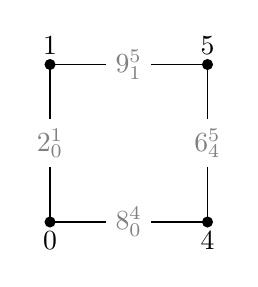
\begin{tikzpicture}[scale=2.0]

\coordinate (0) at (0,0);
\coordinate (4) at (1,0);
\coordinate (1) at (0,1);
\coordinate (5) at (1,1);

\foreach \i in {0,4}
    \fill (\i) circle (1pt) node [below] {\i};

\foreach \i in {1,5}
    \fill (\i) circle (1pt) node [above] {\i};

\draw (0) --(4) -- (5) -- (1) -- (0);



\draw (0.0,  0.5)  node [fill=white, text=gray] {$2_0^1$};
\draw (1.0,  0.5)  node [fill=white, text=gray] {$6_4^5$};
\draw (0.5,  0.0)  node [fill=white, text=gray] {$8_0^4$};
\draw (0.5,  1.0)  node [fill=white, text=gray] {$9_1^5$};

\end{tikzpicture}

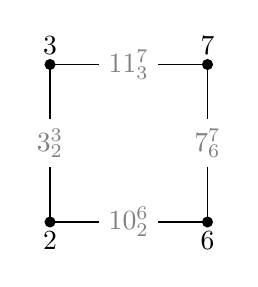
\begin{tikzpicture}[scale=2.0]

\coordinate (2) at (0,0);
\coordinate (6) at (1,0);
\coordinate (3) at (0,1);
\coordinate (7) at (1,1);

\foreach \i in {2,6}
    \fill (\i) circle (1pt) node [below] {\i};

\foreach \i in {3,7}
    \fill (\i) circle (1pt) node [above] {\i};

\draw (2) --(6) -- (7) -- (3) -- (2);



\draw (0.0,  0.5)  node [fill=white, text=gray] {$3_2^3$};
\draw (1.0,  0.5)  node [fill=white, text=gray] {$7_6^7$};
\draw (0.5,  0.0)  node [fill=white, text=gray] {$10_2^6$};
\draw (0.5,  1.0)  node [fill=white, text=gray] {$11_3^7$};

\end{tikzpicture}
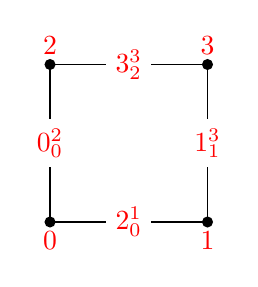
\begin{tikzpicture}[scale=2.0]

\coordinate (0) at (0,0);
\coordinate (1) at (1,0);
\coordinate (2) at (0,1);
\coordinate (3) at (1,1);

\foreach \i in {0,1}
    \fill  [text=red]  (\i) circle (1pt) node [below] {\i};

\foreach \i in {2,3}
    \fill  [text=red]  (\i) circle (1pt) node [above] {\i};

\draw (0) --(1) -- (3) -- (2) -- (0);



\draw (0.0,  0.5)  node [fill=white, text=red] {$0_0^2$};
\draw (1.0,  0.5)  node [fill=white, text=red] {$1_1^3$};
\draw (0.5,  0.0)  node [fill=white, text=red] {$2_0^1$};
\draw (0.5,  1.0)  node [fill=white, text=red] {$3_2^3$};

\end{tikzpicture}
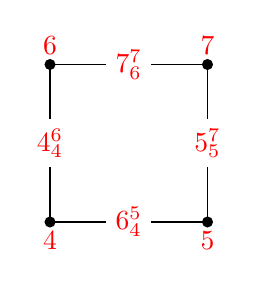
\begin{tikzpicture}[scale=2.0]

\coordinate (4) at (0,0);
\coordinate (5) at (1,0);
\coordinate (6) at (0,1);
\coordinate (7) at (1,1);

\foreach \i in {4,5}
    \fill  [text=red]  (\i) circle (1pt) node [below] {\i};

\foreach \i in {7,6}
    \fill  [text=red]  (\i) circle (1pt) node [above] {\i};

\draw (4) --(5) -- (7) -- (6) -- (4);



\draw (0.0,  0.5)  node [fill=white, text=red] {$4_4^6$};
\draw (1.0,  0.5)  node [fill=white, text=red] {$5_5^7$};
\draw (0.5,  0.0)  node [fill=white, text=red] {$6_4^5$};
\draw (0.5,  1.0)  node [fill=white, text=red] {$7_6^7$};

\end{tikzpicture}



\end{minipage}

\end{frame}


\begin{frame}{2D refinement: quadrilateral}

\centering

\begin{minipage}{0.35\textwidth}

\centering
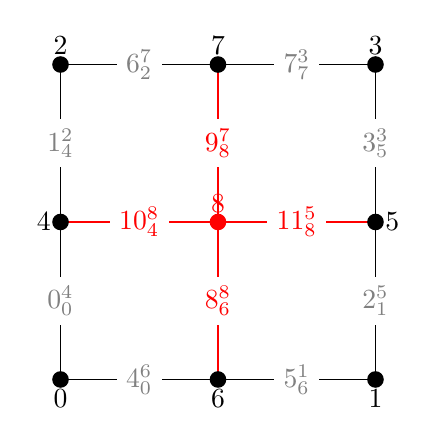
\begin{tikzpicture}[scale=4.0]

\coordinate (0) at (0,0);
\coordinate (1) at (1,0);
\coordinate (2) at (0,1);
\coordinate (3) at (1,1);

\coordinate (4) at (0.0,0.5);
\coordinate (5) at (1.0,0.5);
\coordinate (6) at (0.5,0.0);
\coordinate (7) at (0.5,1.0);

\coordinate (8) at (0.5,0.5);

\draw [red] (4) -- (5);
\draw [red] (6) -- (7);

\foreach \i in {0,1,6}
    \fill  [text=black]  (\i) circle (0.75pt) node [below] {\i};

\foreach \i in {2,3,7}
    \fill  [text=black]  (\i) circle (0.75pt) node [above] {\i};
    
\foreach \i in {4}
    \fill  [text=black]  (\i) circle (0.75pt) node [left] {\i};
    
\foreach \i in {5}
    \fill  [text=black]  (\i) circle (0.75pt) node [right] {\i};

\draw (0) --(1) -- (3) -- (2) -- (0);

\foreach \i in {8}
    \fill  [red, text=red]  (\i) circle (0.75pt) node [above] {\i};


\draw (0.0,  0.25)  node [fill=white, text=gray] {$0_0^4$};
\draw (0.0,  0.75)  node [fill=white, text=gray] {$1_4^2$};
\draw (1.0,  0.25)  node [fill=white, text=gray] {$2_1^5$};
\draw (1.0,  0.75)  node [fill=white, text=gray] {$3_5^3$};

\draw (0.25,  0.0)  node [fill=white, text=gray] {$4_0^6$};
\draw (0.75,  0.0)  node [fill=white, text=gray] {$5_6^1$};
\draw (0.25,  1.0)  node [fill=white, text=gray] {$6_2^7$};
\draw (0.75,  1.0)  node [fill=white, text=gray] {$7_7^3$};

\draw (0.5,  0.25)  node [fill=white, text=red] {$8_6^8$};
\draw (0.5,  0.75)  node [fill=white, text=red] {$9_8^7$};
\draw (0.25,  0.5)  node [fill=white, text=red] {$10_4^8$};
\draw (0.75,  0.5)  node [fill=white, text=red] {$11_8^5$};

\end{tikzpicture}

\end{minipage}
\qquad\qquad
\begin{minipage}{0.45\textwidth}

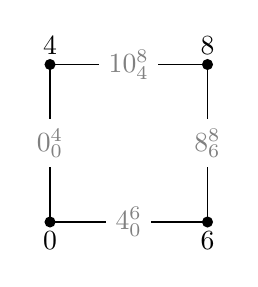
\begin{tikzpicture}[scale=2.0]

\coordinate (0) at (0,0);
\coordinate (6) at (1,0);
\coordinate (4) at (0,1);
\coordinate (8) at (1,1);

\foreach \i in {0,6}
    \fill  [text=black]  (\i) circle (1pt) node [below] {\i};

\foreach \i in {4,8}
    \fill  [text=black]  (\i) circle (1pt) node [above] {\i};

\draw (0) --(6) -- (8) -- (4) -- (0);

\draw (0.0,  0.5)  node [fill=white, text=gray] {$0_0^4$};
\draw (1.0,  0.5)  node [fill=white, text=gray] {$8_6^8$};
\draw (0.5,  0.0)  node [fill=white, text=gray] {$4_0^6$};
\draw (0.5,  1.0)  node [fill=white, text=gray] {$10_4^8$};

\end{tikzpicture}
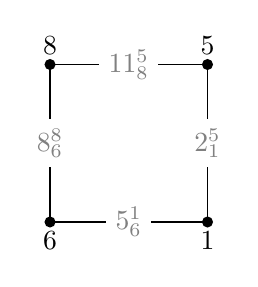
\begin{tikzpicture}[scale=2.0]

\coordinate (6) at (0,0);
\coordinate (1) at (1,0);
\coordinate (8) at (0,1);
\coordinate (5) at (1,1);

\foreach \i in {6,1}
    \fill  [text=black]  (\i) circle (1pt) node [below] {\i};

\foreach \i in {8,5}
    \fill  [text=black]  (\i) circle (1pt) node [above] {\i};

\draw (6) --(1) -- (5) -- (8) -- (6);

\draw (0.0,  0.5)  node [fill=white, text=gray] {$8_6^8$};
\draw (1.0,  0.5)  node [fill=white, text=gray] {$2_1^5$};
\draw (0.5,  0.0)  node [fill=white, text=gray] {$5_6^1$};
\draw (0.5,  1.0)  node [fill=white, text=gray] {$11_8^5$};

\end{tikzpicture}

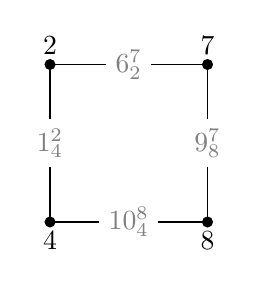
\begin{tikzpicture}[scale=2.0]

\coordinate (4) at (0,0);
\coordinate (8) at (1,0);
\coordinate (2) at (0,1);
\coordinate (7) at (1,1);

\foreach \i in {4,8}
    \fill  [text=black]  (\i) circle (1pt) node [below] {\i};

\foreach \i in {2,7}
    \fill  [text=black]  (\i) circle (1pt) node [above] {\i};

\draw (4) --(8) -- (7) -- (2) -- (4);

\draw (0.0,  0.5)  node [fill=white, text=gray] {$1_4^2$};
\draw (1.0,  0.5)  node [fill=white, text=gray] {$9_8^7$};
\draw (0.5,  0.0)  node [fill=white, text=gray] {$10_4^8$};
\draw (0.5,  1.0)  node [fill=white, text=gray] {$6_2^7$};

\end{tikzpicture}
\begin{tikzpicture}[scale=2.0]

\coordinate (8) at (0,0);
\coordinate (5) at (1,0);
\coordinate (7) at (0,1);
\coordinate (3) at (1,1);

\foreach \i in {8,5}
    \fill  [text=black]  (\i) circle (1pt) node [below] {\i};

\foreach \i in {7,3}
    \fill  [text=black]  (\i) circle (1pt) node [above] {\i};

\draw (8) --(5) -- (3) -- (7) -- (8);

\draw (0.0,  0.5)  node [fill=white, text=gray] {$9_8^7$};
\draw (1.0,  0.5)  node [fill=white, text=gray] {$3_5^3$};
\draw (0.5,  0.0)  node [fill=white, text=gray] {$11_8^5$};
\draw (0.5,  1.0)  node [fill=white, text=gray] {$7_7^3$};

\end{tikzpicture}

\end{minipage}

\end{frame}


\begin{frame}{2D refinement: triangle}

\centering

\begin{minipage}{0.35\textwidth}

\centering
\begin{tikzpicture}[scale=4.5]

\coordinate (0) at (0,0);
\coordinate (1) at (1,0);
\coordinate (2) at (0.5,0.86603);
\coordinate (3) at (0.5,  0.0);
\coordinate (4) at (0.75000,   0.43301);
\coordinate (5) at (0.25000,   0.43301);

\draw [red] (3) --(4) -- (5) -- (3);

\foreach \i in {0,1,3}
    \fill (\i) circle (0.75pt) node [below] {\i};

\foreach \i in {2, 4, 5}
    \fill (\i) circle (0.75pt) node [above] {\i};

\draw (0) --(1) -- (2) -- (0);


\draw (0.25,  0.0)  node [fill=white, text=gray] {$0_0^3$};
\draw (0.75,  0.0)  node [fill=white, text=gray] {$1_3^1$};
\draw (0.875,  0.2165075)  node [fill=white, text=gray] {$2_1^4$};
\draw (0.625,  0.6495225)  node [fill=white, text=gray] {$3_4^2$};
\draw (0.375,  0.6495225)  node [fill=white, text=gray] {$4_2^5$};
\draw (0.125,  0.2165075)  node [fill=white, text=gray] {$5_5^0$};


\draw (0.625,  0.2165075)  node [fill=white, text=red] {$6_3^4$};
\draw (0.500,  0.4330150)  node [fill=white, text=red] {$7_4^5$};
\draw (0.375,  0.2165075)  node [fill=white, text=red] {$8_5^3$};

%\draw (0.75000,   0.43301)  node [fill=white, text=black] {$1_1^2$};
%\draw (0.25000,   0.43301)  node [fill=white, text=black] {$2_2^0$};

\end{tikzpicture}

\end{minipage}
\qquad\qquad
\begin{minipage}{0.45\textwidth}

\begin{tikzpicture}[scale=2.0]

\coordinate (0) at (0,0);
\coordinate (3) at (1,0);
\coordinate (5) at (0.5,0.86603);

\foreach \i in {0,3}
    \fill (\i) circle (1pt) node [below] {\i};

\foreach \i in {5}
    \fill (\i) circle (1pt) node [above] {\i};

\draw (0) --(3) -- (5) -- (0);


\draw (0.5,  0.0)  node [fill=white, text=gray] {$0_3^1$};
\draw (0.75000,   0.43301)  node [fill=white, text=gray] {$8_3^5$};
\draw (0.25000,   0.43301)  node [fill=white, text=gray] {$5_5^0$};

\end{tikzpicture}
\begin{tikzpicture}[scale=2.0]

\coordinate (3) at (0,0);
\coordinate (1) at (1,0);
\coordinate (4) at (0.5,0.86603);

\foreach \i in {3,1}
    \fill (\i) circle (1pt) node [below] {\i};

\foreach \i in {4}
    \fill (\i) circle (1pt) node [above] {\i};

\draw (3) --(1) -- (4) -- (3);


\draw (0.5,  0.0)  node [fill=white, text=gray] {$1_3^1$};
\draw (0.75000,   0.43301)  node [fill=white, text=gray] {$2_1^4$};
\draw (0.25000,   0.43301)  node [fill=white, text=gray] {$6_4^3$};

\end{tikzpicture}

\begin{tikzpicture}[scale=2.0]

\coordinate (5) at (0,0);
\coordinate (4) at (1,0);
\coordinate (2) at (0.5,0.86603);

\foreach \i in {5,4}
    \fill (\i) circle (1pt) node [below] {\i};

\foreach \i in {2}
    \fill (\i) circle (1pt) node [above] {\i};

\draw (5) --(4) -- (2) -- (5);


\draw (0.5,  0.0)  node [fill=white, text=gray] {$7_4^4$};
\draw (0.75000,   0.43301)  node [fill=white, text=gray] {$3_4^2$};
\draw (0.25000,   0.43301)  node [fill=white, text=gray] {$4_2^5$};

\end{tikzpicture}
\begin{tikzpicture}[scale=2.0]

\coordinate (3) at (0,0);
\coordinate (4) at (1,0);
\coordinate (5) at (0.5,0.86603);

\foreach \i in {3,4}
    \fill (\i) circle (1pt) node [below] {\i};

\foreach \i in {5}
    \fill (\i) circle (1pt) node [above] {\i};

\draw (3) --(4) -- (5) -- (3);


\draw (0.5,  0.0)  node [fill=white, text=gray] {$6_3^4$};
\draw (0.75000,   0.43301)  node [fill=white, text=gray] {$7_4^5$};
\draw (0.25000,   0.43301)  node [fill=white, text=gray] {$8_5^3$};

\end{tikzpicture}

\end{minipage}

\end{frame}



\end{document}